% !TEX root = ../report.tex

\section{Project management}\label{plan}
\thispagestyle{plain}

\subsection{Project structure}\label{plan/structure}

At a high level, the project was structured as a team within a hypothetical
engineering consultancy being commissioned to undertake the project. This creates
several key roles both within and outside of the team, including a sponsor, a
supervisor, a project manager, and one or more consultants. The sponsor of the
project, Dr John Levine, provided the topic and the initial aims of the
project, but has no formal role in the project as it develops, except for
clarification of requirements and recommendations for design decisions.

The team supervisor, Dr Marilyn Lennon, serves as an advisor and manager of
the team, providing guidance in project management and general engineering
guidance, though without in-depth technical knowledge of the subject matter.
This role is very useful, as it enforces good engineering practices and
project structure, while preventing the project management from being
inhibited by details overly specific to the project.

Since the supervisor does not have all the technical knowledge the team
requires, other academics will take on the role of consultants, allowing the
team access to in-depth specialist knowledge. Examples of consultants who have
already contributed advice to the project are Dr Mark Post and Dr James Irvine,
who have supplied insight into practical robotics and microcontrollers,
respectively. This also has the benefit that,
while the team retains access to the expertise of the consultants, they are not
formally part of the project, so the team still has the final judgement in
design decisions.

Within the team, a project manager was appointed. The manager is not a team
leader, and has no increased authority over design decisions, but assigns tasks
and enforces deadlines on the whole team. This
attempts to ensure each team member is able to contribute to decisions made by
the group, and that all options are given equal consideration. It also imposes
order on the structure of the team while minimising needless bureaucracy.

\subsection{Project workflow}\label{plan/workflow}

All files relevant to the project are stored on a GitHub repository for
version control and access by all team members. The master branch cannot be
modified except by branch merging, so team members must work on their own
branches, and another team member must approve changes to allow them to be
finalised.

The repository is integrated with Slack, a tool for team communication.
Discussions are either held on Slack, or minutes are uploaded to Slack.
Tasks are created during meetings and posted as issues on GitHub immediately.
Each task is attributed to team members on a voluntary basis, and failing
that by assignment by the project manager.

\subsection{Objectives}\label{plan/objectives}

The specific objectives of this project were as follows:
\begin{itemize}
    \item{Design a simple differential drive robot capable of exploring and perceiving its environment---Major Objective (Source: Section~\ref{design/mechanical/conclusion})}
    \item{Construct two robots using this design---Major Objective (Source:~\ref{introduction/context})}
    \item{Develop SLAM algorithm to allow the robots to explore an area---Major Objective (Source: Section~\ref{design/software/conclusion})}
    \item{Develop a system to allow the robots to interact and communicate with each other---Major Objective (Source: Section~\ref{design/software/conclusion})}
    \item{Develop algorithms to search a maze which can be dynamically parallelised over any number of agents---Major Objective (Source: Section~\ref{design/software/conclusion})}
    \item{Develop a test environment and evaluate the robots’ performance---Major Objective (Source: Section~\ref{introduction/context})}
    \item{Add additional robot(s) and evaluate scalability of approach---Optional Objective(Source: Section~\ref{introduction/context})}
    \item{Improve SLAM by adding loop closure between robots---Optional Objective (Source: Section~\ref{background/slam})}
\end{itemize}

\subsection{Risk evaluation}\label{plan/riskeval}
The main technical risks of the project initially revolve around possible lead times for the ordering of parts. This will be mitigated by ordering parts as soon as feasibly possible and also by carrying out other work such as research and further design planning in the interim. Following on from this, components will also form the main aspect of technical risk in the latter stages of the project such as if a part is damaged or stops working. In order to mitigate this risk, time is left at the end of the project where no parts are being worked on directly and so it is unlikely for components to be broken. Time for testing, evaluation and report writing can also be used to order new components in serious cases. For components with extensive lead times in the first instance, spares may be ordered---if not too expensive---to further eliminate this risk.


\subsection{Timeline}\label{plan/timeline}

The Gantt chart here Figure~\ref{figure:gantt} was created using the objectives determined in each section of the design (Section~\ref{design}). The timescales were determined approximately using knowledge obtained from research with the addition of time for possible technical risks. These were considered carefully and an agile method was adopted in order to allow the tasks to be completed and give a small margin of error within the Gantt chart. For example, assembly of remaining robots is allocated a longer time than expected as this will involved lead times for components and also spans the period of time when the labs will be closed and construction work may not be possible.

Figure~\ref{figure:gantt} shows a Gantt chart of the project timeline.


\begin{landscape} % Rotates the image on the page
\global\pdfpageattr\expandafter{\the\pdfpageattr/Rotate 90} % Rotates the page in the PDF output
\begin{figure}[!p]\centering
    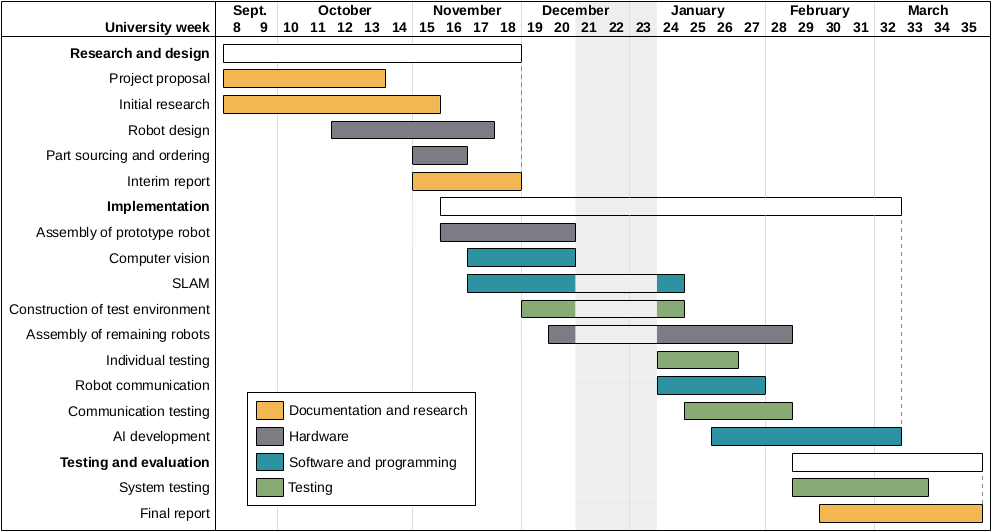
\includegraphics[width=1\linewidth]{gantt}
    \caption{Gantt chart}\label{figure:gantt}
\end{figure}
\end{landscape}
\global\pdfpageattr\expandafter{\the\pdfpageattr/Rotate 0}
